\chapter{適用例}\label{cha:Indication}
本章では、本研究で作成したモータ特性表自動生成ツールが正しく動作することを検証するため、以下の2種類のModelicaモデルのシミュレーション結果のcsvファイルを適用する。
\begin{itemize}
    \item ブラシ付きDCモータのModelicaモデル
    \item ブラシ付きDCモータのModelicaモデルをサブシステムとするモデル
\end{itemize}
% 2つのモデルのパラメータ設定を以下に示す。
% \begin{itemize}
%     \item 電源部品 ・・・ 9 V
%     \item 抵抗部品 ・・・ 1.78 $\Omega$
%     \item インダクタ部品 ・・・ 0.0000735 H
%     \item 起電力部品 ・・・ 0.010400000000000001 $mN \cdot m$
%     \item 慣性部品 ・・・ 0.00371135959 $\mathrm{kg\cdot m^2}$
% \end{itemize}
具体的には、以下の2つの項目を確認する。
\begin{enumerate}
    \item 生成したモータ特性表の各要素の値が、正しい値になっていること
    \item 2つのモデルから生成したモータ特性表の各要素が、同値になっていること
\end{enumerate}
\section{ブラシ付きDCモータのModelicaモデル}
ブラシ付きDCモータのModelicaモデルから生成したcsvファイルを、モータ特性表自動生成ツールに適用する。適用例に用いるモデルを、図\ref{fig:tekiyou_tanntai}に、
図\ref{fig:tekiyou_mortoku}のシミュレーション結果であるcsvファイルの一部を、図\ref{fig:tekiyou_csv}にそれぞれ示す。
\begin{figure}[t]
	\centering
	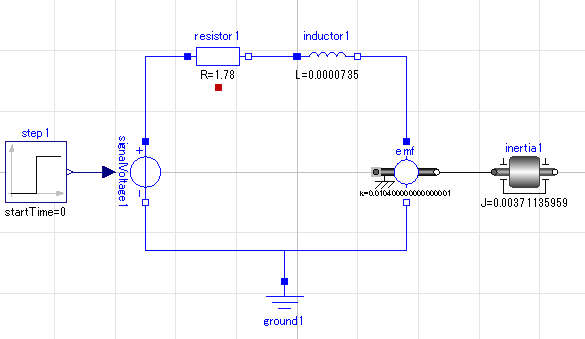
\includegraphics[width=10cm]{./Image/tekiyou_tanntai.png}
	\caption{適用するブラシ付きDCモータのModelicaモデル}
	\label{fig:tekiyou_tanntai}
\end{figure}
\begin{figure}[t]
	\centering
	\fbox{
    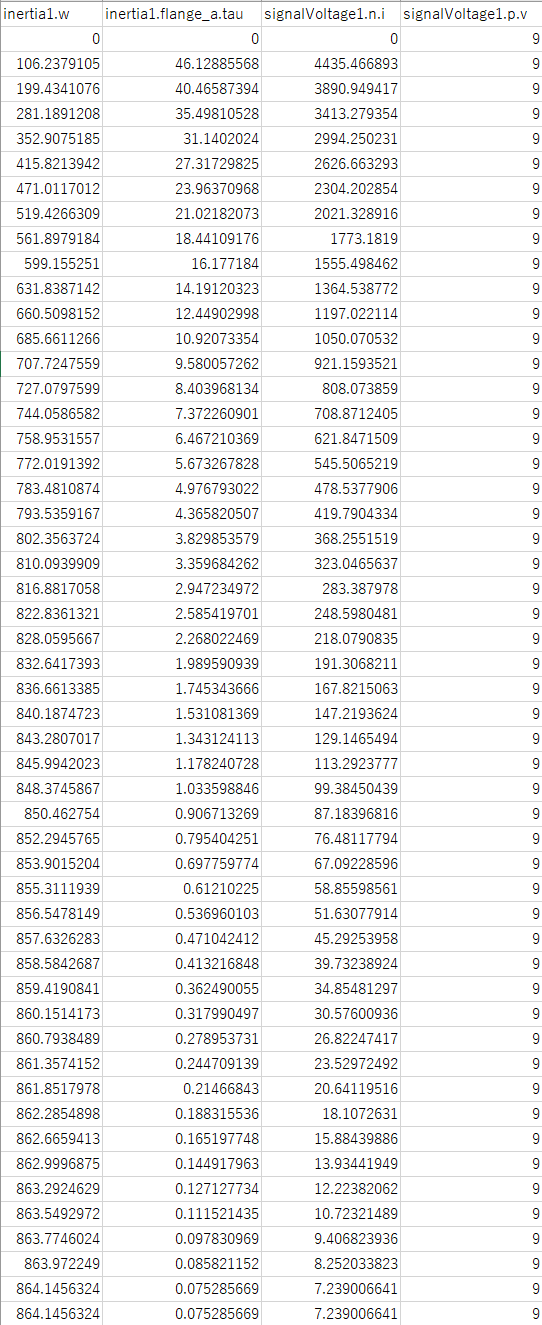
\includegraphics[width=9cm]{./Image/tekiyou_csv.png}
    }
    \caption{図\ref{fig:tekiyou_mortoku}のシミュレーション結果であるcsvファイルの一部}
	\label{fig:tekiyou_csv}
\end{figure}
図\ref{fig:tekiyou_csv}のcsvファイルをモータ特性表自動生成ツールに適用した結果、出力するモータ特性表を図\ref{fig:tekiyou_mortoku}に示す。
\begin{figure}[t]
	\centering
	\fbox{
    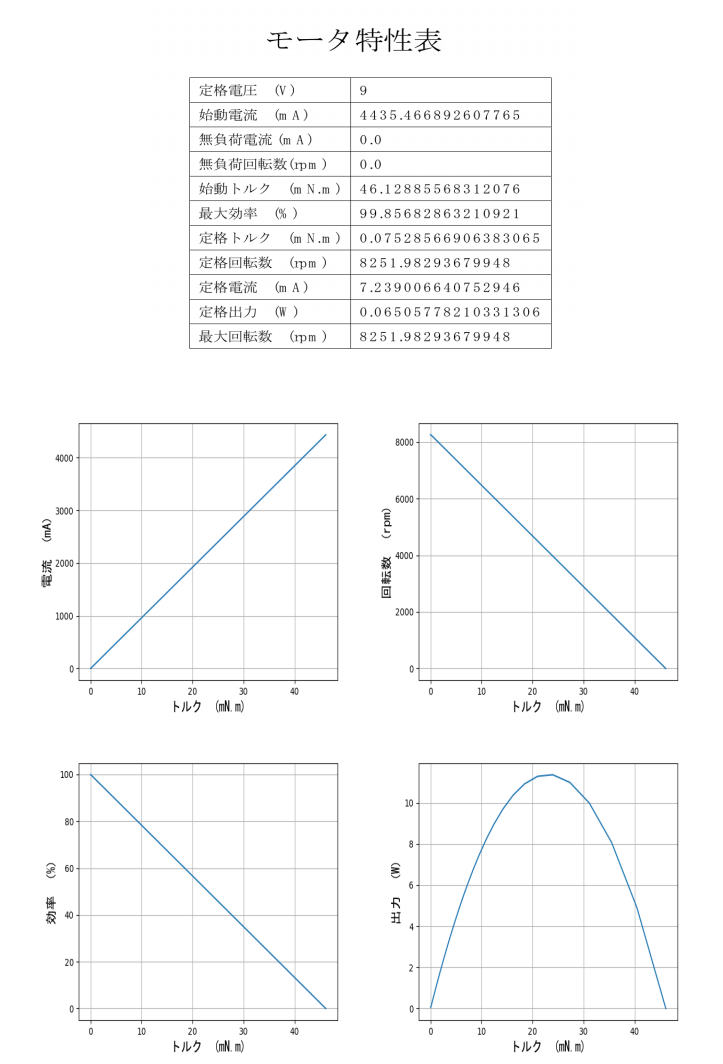
\includegraphics[width=14cm]{./Image/tekiyou_mortoku.png}
    }
    \caption{適用例で生成したモータ特性表}
	\label{fig:tekiyou_mortoku}
\end{figure}

\clearpage
\subsection{特性表の確認}
以下に、特性表で出力した各要素が正しく算出できているか確認する。
\subsubsection{電圧}
図\ref{fig:tekiyou_mortoku}の特性表にある電圧の値と、図\ref{fig:tekiyou_csv}のsignalVoltage1.p.vが持つ値の中で、先頭にある値が同値である。よって、正しく出力していることが確認できる。
\subsubsection{始動電流}
図\ref{fig:tekiyou_mortoku}の特性表にある始動電流の値と、図\ref{fig:tekiyou_csv}のsignalVoltage1.n.iが持つ値の中の最大値が同値である。よって、正しく出力していることが確認できる。
\subsubsection{停動トルク}
図\ref{fig:tekiyou_mortoku}の特性表にある停動トルクの値と、図\ref{fig:tekiyou_csv}のinertia1.flange\_a.tauが持つ値の中の最大値が同値である。よって、正しく出力していることが確認できる。
\subsubsection{最大効率}
図\ref{fig:tekiyou_mortoku}の特性表にある最大効率の値と、図\ref{fig:tekiyou_csv}の効率が持つ値の中の最大値が同値である。よって、正しく出力していることが確認できる。
\subsubsection{定格トルク}
図\ref{fig:tekiyou_mortoku}の特性表にある定格トルクの値と、図\ref{fig:tekiyou_csv}のトルクが持つ値の中の、最大効率を出した時の値が同値である。よって、正しく出力していることが確認できる。
\subsubsection{定格回転数}
図\ref{fig:tekiyou_mortoku}の特性表にある定格回転数の値と、図\ref{fig:tekiyou_csv}の回転数が持つ値の中の、最大効率を出した時の値が同値である。よって、正しく出力していることが確認できる。
\subsubsection{定格電流}
図\ref{fig:tekiyou_mortoku}の特性表にある定格電流と、図\ref{fig:tekiyou_csv}の電流が持つ値の中の、最大効率を出した時の値が同値である。よって、正しく出力していることが確認できる。
\subsubsection{定格出力}
図\ref{fig:tekiyou_mortoku}の特性表にある定格出力と、図\ref{fig:tekiyou_csv}の出力が持つ値の中の、最大効率を出した時の値が同値である。よって、正しく出力していることが確認できる。
\subsubsection{最大回転数}
図\ref{fig:tekiyou_mortoku}の特性表にある最大回転数と、図\ref{fig:tekiyou_csv}の回転数が持つ値の中の最大値が同値である。よって、正しく出力していることが確認できる。
\subsection{特性グラフの確認}
以下に、特性グラフが正しく生成できているか確認する。

\section{ブラシ付きDCモータのModelicaモデルをサブシステムとするモデル}
